\documentclass[border=6pt,tikz]{standalone}
\usepackage{amsmath,amssymb}
\usepackage{microtype}
\usetikzlibrary{arrows.meta,positioning,calc,shapes.geometric,fit,backgrounds}

% Academic Color Palette (MLSys/ICLR Style)
\definecolor{sinkgreen}{RGB}{240, 253, 244}
\definecolor{sinkgreenborder}{RGB}{22, 163, 74}
\definecolor{quantblue}{RGB}{239, 246, 255}
\definecolor{quantblueborder}{RGB}{37, 99, 235}
\definecolor{tailteal}{RGB}{240, 253, 250}
\definecolor{tailtealborder}{RGB}{13, 148, 136}
\definecolor{convred}{RGB}{254, 242, 242}
\definecolor{convredborder}{RGB}{220, 38, 38}
\definecolor{pgpurple}{RGB}{245, 243, 255}
\definecolor{pgpurpleborder}{RGB}{124, 58, 237}
\definecolor{hardwaregray}{RGB}{248, 250, 252}
\definecolor{hardwaregrayborder}{RGB}{100, 116, 139}
\definecolor{mathdark}{RGB}{15, 23, 42}
\definecolor{goldaccent}{RGB}{217, 119, 6}
\definecolor{goldbg}{RGB}{254, 252, 232}

\begin{document}
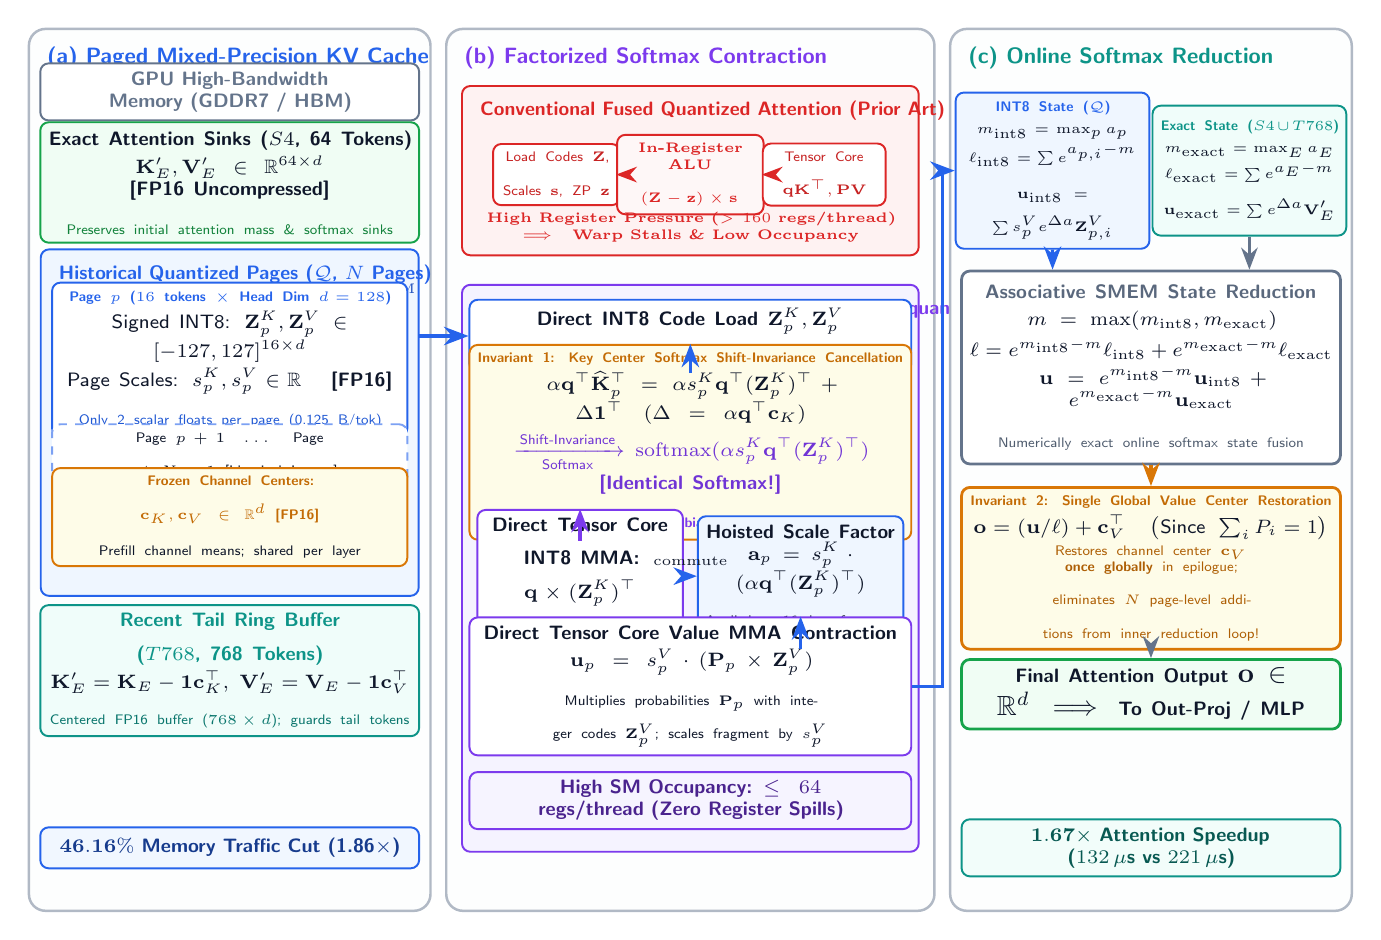
\begin{tikzpicture}[
    font=\sffamily,
    >=Stealth,
    every node/.style={align=center, color=mathdark},
    panelbg/.style={draw=hardwaregrayborder!50, fill=hardwaregray!30, rounded corners=6pt, line width=0.9pt},
    panelhead/.style={font=\sffamily\bfseries\footnotesize, anchor=north west, inner sep=4pt},
    card/.style={rounded corners=3pt, line width=0.7pt, inner sep=3pt},
    arr/.style={->, line width=1.1pt, draw=hardwaregrayborder},
    arrblue/.style={->, line width=1.2pt, draw=quantblueborder},
    arrred/.style={->, line width=1pt, draw=convredborder, dashed},
    arrpurple/.style={->, line width=1.2pt, draw=pgpurpleborder},
    arrgold/.style={->, line width=1.2pt, draw=goldaccent}
]

% =========================================================================
% COORDINATE SYSTEM (TOTAL WIDTH: 17.0 cm, HEIGHT: 11.2 cm)
% Panel A: Center X = 2.65, Width = 5.1 (Range: [0.1, 5.2])
% Panel B: Center X = 8.50, Width = 6.2 (Range: [5.4, 11.6])
% Panel C: Center X = 14.35, Width = 5.1 (Range: [11.8, 16.9])
% =========================================================================

% -------------------------------------------------------------------------
% PANEL (A): PAGED MIXED-PRECISION KV CACHE HIERARCHY
% -------------------------------------------------------------------------
\node[panelbg, minimum width=5.1cm, minimum height=11.2cm] (panelA) at (2.65, 0) {};
\node[panelhead, text=quantblueborder] at ($(panelA.north west)+(0.1,-0.1)$) {
    (a) Paged Mixed-Precision KV Cache
};

% GPU HBM Tier
\node[card, draw=hardwaregrayborder, fill=white, font=\sffamily\bfseries\scriptsize, text=hardwaregrayborder,
      text width=4.6cm, minimum height=0.48cm] (hbm) at (2.65, 4.8) {
    GPU High-Bandwidth Memory (GDDR7 / HBM)
};

% 1. Prefix Sinks S4
\node[card, draw=sinkgreenborder, fill=sinkgreen, text width=4.6cm, minimum height=1.3cm] (sink) at (2.65, 3.65) {
    \textbf{\scriptsize Exact Attention Sinks ($S4$, 64 Tokens)}\\[1pt]
    \scriptsize $\mathbf{K}'_E, \mathbf{V}'_E \in \mathbb{R}^{64 \times d}$ \quad \textbf{[FP16 Uncompressed]}\\[2pt]
    \tiny\color{sinkgreenborder!80!black} Preserves initial attention mass \& softmax sinks
};

% 2. Historical Quantized Pages Q
\node[card, draw=quantblueborder, fill=quantblue, minimum width=4.8cm, minimum height=4.4cm] (quant) at (2.65, 0.6) {};
\node[anchor=north west, font=\sffamily\bfseries\scriptsize, text=quantblueborder] at ($(quant.north west)+(0.12,-0.08)$) {
    Historical Quantized Pages ($\mathcal{Q}$, $N$ Pages)
};
\node[anchor=north west, font=\tiny, text=quantblueborder!80!black] at ($(quant.north west)+(0.12,-0.32)$) {
    Paged buffer: $P=16$ tokens/page in HBM
};

% Page p breakdown
\node[card, draw=quantblueborder, fill=white, text width=4.3cm, minimum height=1.65cm] (pageP) at (2.65, 1.4) {
    \textbf{\tiny\color{quantblueborder} Page $p$ ($16$ tokens $\times$ Head Dim $d=128$)}\\[2pt]
    \scriptsize Signed INT8: $\mathbf{Z}_p^K, \mathbf{Z}_p^V \in [-127, 127]^{16 \times d}$\\[1pt]
    \scriptsize Page Scales: $s_p^K, s_p^V \in \mathbb{R}$ \quad \textbf{[FP16]}\\[2pt]
    \tiny\color{quantblueborder!90!black} Only 2 scalar floats per page (0.125 B/tok)
};

% Page p+1 ellipsis
\node[card, draw=quantblueborder!60, fill=white, dashed, text width=4.3cm, minimum height=0.42cm] (pageP1) at (2.65, 0.18) {
    \tiny Page $p+1 \quad \dots \quad$ Page $p+N-1$ [Identical Layout]
};

% Frozen Global Centers
\node[card, draw=goldaccent, fill=goldbg, text width=4.3cm, minimum height=0.75cm] (centers) at (2.65, -0.6) {
    \textbf{\tiny\color{goldaccent!90!black} Frozen Channel Centers: $\mathbf{c}_K, \mathbf{c}_V \in \mathbb{R}^d$ [FP16]}\\[1pt]
    \tiny Prefill channel means; shared per layer
};

% 3. Recent Tail Ring Buffer
\node[card, draw=tailtealborder, fill=tailteal, text width=4.6cm, minimum height=1.3cm] (tail) at (2.65, -2.55) {
    \textbf{\scriptsize\color{tailtealborder} Recent Tail Ring Buffer ($T768$, 768 Tokens)}\\[1pt]
    \scriptsize $\mathbf{K}'_E = \mathbf{K}_E - \mathbf{1}\mathbf{c}_K^\top, \; \mathbf{V}'_E = \mathbf{V}_E - \mathbf{1}\mathbf{c}_V^\top$\\[1pt]
    \tiny\color{tailtealborder!80!black} Centered FP16 buffer ($768 \times d$); guards tail tokens
};

% Bandwidth saving badge
\node[card, draw=quantblueborder, fill=quantblue!90!white, text=quantblueborder!60!black, font=\sffamily\bfseries\scriptsize,
      text width=4.6cm, minimum height=0.52cm] (saving) at (2.65, -4.8) {
    $\mathbf{46.16\%}$ Memory Traffic Cut (1.86$\times$)
};


% -------------------------------------------------------------------------
% PANEL (B): FACTORIZED SOFTMAX CONTRACTION PIPELINE
% -------------------------------------------------------------------------
\node[panelbg, minimum width=6.2cm, minimum height=11.2cm] (panelB) at (8.5, 0) {};
\node[panelhead, text=pgpurpleborder] at ($(panelB.north west)+(0.1,-0.1)$) {
    (b) Factorized Softmax Contraction
};

% Top: Conventional Fused Baseline (Stalls)
\node[card, draw=convredborder, fill=convred, minimum width=5.8cm, minimum height=2.15cm] (convBox) at (8.5, 3.8) {};
\node[anchor=north west, font=\sffamily\bfseries\scriptsize, text=convredborder] at ($(convBox.north west)+(0.12,-0.08)$) {
    Conventional Fused Quantized Attention (Prior Art)
};

\node[card, draw=convredborder, fill=white, text=convredborder!90!black, text width=1.4cm, minimum height=0.72cm] (cLoad) at (6.8, 3.75) {
    \tiny Load Codes $\mathbf{Z}$,\\Scales $\mathbf{s}$, ZP $\mathbf{z}$
};
\node[card, draw=convredborder, fill=convred!60, text=convredborder, font=\bfseries, text width=1.65cm, minimum height=0.72cm] (cALU) at (8.5, 3.75) {
    \tiny In-Register ALU\\$(\mathbf{Z} - \mathbf{z}) \times \mathbf{s}$
};
\node[card, draw=convredborder, fill=white, text=convredborder!90!black, text width=1.35cm, minimum height=0.72cm] (cMMA) at (10.2, 3.75) {
    \tiny Tensor Core\\$\mathbf{q}\mathbf{K}^\top, \mathbf{P}\mathbf{V}$
};

\draw[arrred] (cLoad) -- (cALU);
\draw[arrred] (cALU) -- (cMMA);

\node[anchor=south, font=\tiny\bfseries, text=convredborder, text width=5.6cm] at ($(convBox.south)+(0, 0.06)$) {
    High Register Pressure ($>160$ regs/thread) $\implies$ Warp Stalls \& Low Occupancy
};

% Bottom: PageGauge Factorized Pipeline
\node[card, draw=pgpurpleborder, fill=pgpurple, minimum width=5.8cm, minimum height=7.2cm] (pgBox) at (8.5, -1.25) {};
\node[anchor=north west, font=\sffamily\bfseries\scriptsize, text=pgpurpleborder] at ($(pgBox.north west)+(0.12,-0.08)$) {
    PageGauge Factorized Execution (Zero ALU Dequantization)
};

% Step 1: Direct Load
\node[card, draw=quantblueborder, fill=white, text width=5.4cm, minimum height=0.62cm] (pgLoad) at (8.5, 1.7) {
    \textbf{\scriptsize Direct INT8 Code Load $\mathbf{Z}_p^K, \mathbf{Z}_p^V$} \quad \scriptsize(\textit{Halves HBM Load Traffic})
};

% Step 2: Shift-Invariance Cancellation Box
\node[card, draw=goldaccent, fill=goldbg, text width=5.4cm, minimum height=1.65cm] (shiftInv) at (8.5, 0.35) {
    \textbf{\tiny\color{goldaccent!90!black} Invariant 1: Key Center Softmax Shift-Invariance Cancellation}\\[2pt]
    \scriptsize $\alpha \mathbf{q}^\top \widehat{\mathbf{K}}_p^\top = \alpha s_p^K \mathbf{q}^\top (\mathbf{Z}_p^K)^\top + \Delta \mathbf{1}^\top \quad (\Delta = \alpha \mathbf{q}^\top \mathbf{c}_K)$\\[2pt]
    \scriptsize\color{pgpurpleborder!90!black} $\xrightarrow[\text{Softmax}]{\text{Shift-Invariance}} \operatorname{softmax}(\alpha s_p^K \mathbf{q}^\top (\mathbf{Z}_p^K)^\top)$ \quad \textbf{[Identical Softmax!]}\\[2pt]
    \tiny\bfseries\color{pgpurpleborder} $\implies$ Zero elementwise bias/subtraction in registers!
};

% Step 3: Direct Tensor Core MMA QK^T & Step 4: Scale Hoisting
\node[card, draw=pgpurpleborder, fill=white, text width=2.4cm, minimum height=1.05cm] (tcQK) at (7.1, -1.35) {
    \textbf{\scriptsize Direct Tensor Core}\\
    \textbf{\scriptsize INT8 MMA: $\mathbf{q} \times (\mathbf{Z}_p^K)^\top$}\\[1pt]
    \tiny Raw code contraction
};

\node[card, draw=quantblueborder, fill=quantblue, text width=2.4cm, minimum height=1.05cm] (scaleHoist) at (9.9, -1.35) {
    \textbf{\scriptsize Hoisted Scale Factor}\\
    \scriptsize $\mathbf{a}_p = s_p^K \cdot (\alpha \mathbf{q}^\top (\mathbf{Z}_p^K)^\top)$\\[1pt]
    \tiny Applied to 16-elem fragment
};

\draw[arrblue] (tcQK) -- (scaleHoist) node[midway, above, font=\tiny] {commute};

% Step 5: Direct TC Value MMA
\node[card, draw=pgpurpleborder, fill=white, text width=5.4cm, minimum height=1.15cm] (tcPV) at (8.5, -2.75) {
    \textbf{\scriptsize Direct Tensor Core Value MMA Contraction}\\[2pt]
    \scriptsize $\mathbf{u}_p = s_p^V \cdot (\mathbf{P}_p \times \mathbf{Z}_p^V)$\\[2pt]
    \tiny Multiplies probabilities $\mathbf{P}_p$ with integer codes $\mathbf{Z}_p^V$; scales fragment by $s_p^V$
};

\draw[arrblue] (pgLoad) -- (shiftInv);
\draw[arrpurple] ($(shiftInv.south)+(-1.4, 0)$) -- (tcQK.north);
\draw[arrblue] (scaleHoist.south) -- ++(0,-0.15) -| ($(tcPV.north)+(1.4, 0)$);

\node[card, draw=pgpurpleborder, fill=pgpurple!90!white, text=pgpurpleborder!60!black, font=\sffamily\bfseries\scriptsize,
      text width=5.4cm, minimum height=0.48cm] at (8.5, -4.2) {
    High SM Occupancy: $\le 64$ regs/thread (Zero Register Spills)
};


% -------------------------------------------------------------------------
% PANEL (C): ONLINE SOFTMAX REDUCTION & CENTER RESTORATION
% -------------------------------------------------------------------------
\node[panelbg, minimum width=5.1cm, minimum height=11.2cm] (panelC) at (14.35, 0) {};
\node[panelhead, text=tailtealborder] at ($(panelC.north west)+(0.1,-0.1)$) {
    (c) Online Softmax Reduction
};

% Side-by-Side Partial States at top of Panel C!
% Left: INT8 State (from Historical Pages Q)
\node[card, draw=quantblueborder, fill=quantblue, text width=2.25cm, minimum height=1.65cm] (stateInt8) at (13.1, 3.8) {
    \textbf{\tiny\color{quantblueborder} INT8 State ($\mathcal{Q}$)}\\[2pt]
    \tiny $m_{\rm int8} = \max_p a_p$\\[1pt]
    \tiny $\ell_{\rm int8} = \sum e^{a_{p,i} - m}$\\[1pt]
    \tiny $\mathbf{u}_{\rm int8} = \sum s_p^V e^{\Delta a} \mathbf{Z}_{p,i}^V$
};

% Right: Exact State (from S4 and T768)
\node[card, draw=tailtealborder, fill=tailteal, text width=2.25cm, minimum height=1.65cm] (stateExact) at (15.6, 3.8) {
    \textbf{\tiny\color{tailtealborder} Exact State ($S4 \cup T768$)}\\[2pt]
    \tiny $m_{\rm exact} = \max_E a_E$\\[1pt]
    \tiny $\ell_{\rm exact} = \sum e^{a_E - m}$\\[1pt]
    \tiny $\mathbf{u}_{\rm exact} = \sum e^{\Delta a} \mathbf{V}'_E$
};

% Associative Online Reduction Box (SMEM)
\node[card, draw=hardwaregrayborder, fill=white, line width=1pt, text width=4.6cm, minimum height=2.45cm] (reducer) at (14.35, 1.3) {
    \textbf{\scriptsize\color{hardwaregrayborder!90!black} Associative SMEM State Reduction}\\[2pt]
    \scriptsize $m = \max(m_{\rm int8}, m_{\rm exact})$\\[2pt]
    \scriptsize $\ell = e^{m_{\rm int8}-m}\ell_{\rm int8} + e^{m_{\rm exact}-m}\ell_{\rm exact}$\\[2pt]
    \scriptsize $\mathbf{u} = e^{m_{\rm int8}-m}\mathbf{u}_{\rm int8} + e^{m_{\rm exact}-m}\mathbf{u}_{\rm exact}$\\[3pt]
    \tiny\color{hardwaregrayborder!80!black} Numerically exact online softmax state fusion
};

\draw[arrblue] (stateInt8.south) -- ($(reducer.north)+(-1.25, 0)$);
\draw[arr] (stateExact.south) -- ($(reducer.north)+(1.25, 0)$);

% Global Value Center Restoration (Epilogue)
\node[card, draw=goldaccent, fill=goldbg, line width=1pt, text width=4.6cm, minimum height=1.75cm] (epilogue) at (14.35, -1.25) {
    \textbf{\tiny\color{goldaccent!90!black} Invariant 2: Single Global Value Center Restoration}\\[2pt]
    \scriptsize $\mathbf{o} = (\mathbf{u} / \ell) + \mathbf{c}_V^\top \quad \left(\text{Since } \sum_i P_i = 1\right)$\\[2pt]
    \tiny\color{goldaccent!80!black} Restores channel center $\mathbf{c}_V$ \textbf{once globally} in epilogue;\\
    eliminates $N$ page-level additions from inner reduction loop!
};

\draw[arrgold] (reducer) -- (epilogue);

% Final Attention Output Vector
\node[card, draw=sinkgreenborder, fill=sinkgreen, line width=1pt, text width=4.6cm, minimum height=0.7cm] (outVec) at (14.35, -2.85) {
    \textbf{\scriptsize Final Attention Output} $\mathbf{o} \in \mathbb{R}^d \implies$ \textbf{\scriptsize To Out-Proj / MLP}
};

\draw[arr] (epilogue) -- (outVec);

% Bottom latency gain badge
\node[card, draw=tailtealborder, fill=tailteal!90!white, text=tailtealborder!60!black, font=\sffamily\bfseries\scriptsize,
      text width=4.6cm, minimum height=0.52cm] at (14.35, -4.8) {
    $\mathbf{1.67\times}$ Attention Speedup ($132\,\mu$s vs $221\,\mu$s)
};

% =========================================================================
% INTER-PANEL DATAFLOW ARROWS (ROUTED IN EMPTY GUTTERS)
% Gutter 1 between A & B: X in [5.2, 5.4]
% Gutter 2 between B & C: X in [11.6, 11.8]
% =========================================================================
\draw[arrblue, line width=1.3pt] (5.05, 1.7) -- (pgLoad.west);
\draw[arrblue, line width=1.3pt] (tcPV.east) -- (11.7, -2.75) -- (11.7, 3.8) -- (stateInt8.west);

\end{tikzpicture}
\end{document}
